\chapter{Networking Model Attributes}\label{app:attributes}

\section{Central Server Model}
\begin{figure}[!h]
  \begin{tabular}{ c p{0.94\textwidth} }
    \faCheckCircle & Hardware is likely to be powerful enough to handle the stress of many simulations running simultaneously. \\
    \faCheckCircle & High bandwidth connection is likely to be used. Minimises the chance of high latency and network issues. \\
    \faCheckCircle & Ping to the server is likely to be similar for all players making the game more fair.  \\
    \faCheckCircle & No client can see the address of any other client. \\
    \faCheckCircle & The developer has a lot of control over what is allowed within the game. This allows for anti-cheating systems that are hard to bypass. \\
    \  & \  \\
    \faTimesCircle & Expensive to rent out, or buy and maintain, server space. Letting players rent out servers makes the game more expensive for them. \\
    \faTimesCircle & Many servers have to be spread out evenly throughout the world to allow for low latency connections.  \\
    \faTimesCircle & People living in remote locations may not have low latency access to official servers.
  \end{tabular}
  \caption{The attributes of the central server model}
  \label{fig:cs_attributes}
\end{figure}

\newpage

\section{Client Hosted Model}
\begin{figure}[!h]
  \begin{tabular}{ c p{0.94\textwidth} }
    \faCheckCircle & There are no additional costs to the publisher/developer when releasing the game. \\
    \faCheckCircle & Players in remote locations can play together with low latency. \\
    \faCheckCircle & The codebase is relatively easily transferable to a central server model if the need arises. \\
    \  & \  \\
    \faTimesCircle & The host player has negligible ping to the server. This could be a large advantage.  \\
    \faTimesCircle & The host player is likely to use a consumer grade connection increasing the risk of packet loss and high latency \\
    \faTimesCircle & The host player could be using WiFi to host the game which could significantly increase the chance of packet loss. \\
    \faTimesCircle & The host's hardware may not be powerful enough to calculate each simulation step within an acceptable tick rate. \\
    \faTimesCircle & If the host player is disconnected mid-game, a host migration will have to take place pausing the game for a few seconds or causing the game to finish unexpectedly. \\
    \faTimesCircle & The host player can see the IP address of each other player that they are playing with. \\
    \faTimesCircle & Cheating could be easy if the host player sends malicious packets to the clients pretending to be the game server.

  \end{tabular}
  \caption{The attributes of the client hosted model}
  \label{fig:ch_attributes}
\end{figure}

\newpage

\section{Peer to Peer model}
\begin{figure}[!h]
  \begin{tabular}{ c p{0.94\textwidth} }
    \faCheckCircle & There are no additional costs to the publisher/developer when releasing the game. \\
    \faCheckCircle & Players in remote locations can play together with low latency. \\
    \faCheckCircle & There is no concept of host advantage, like what is present with the client hosted model. \\
    \faCheckCircle & Host migrations are not a large problem since everyone has the full simulation state. \\
    \  & \  \\
    \faMinusCircle & Each client communicates directly with other clients making their connection as efficient as possible in theory. \\
    \faMinusCircle & Even though a central ``authority'' is not needed, one of the peers often has to act as a session host to handle invitations and handshakes. \\
    \faMinusCircle & Every client runs it's own simulation and is tasked with keeping it updated with everyone else's. \\
    \  & \  \\
    \faTimesCircle & The lack of a central authority (such as a game server) makes cheat prevention difficult. \\
    \faTimesCircle & Each player in an instance, can see the IP address of every other player they are playing with. \\
    \faTimesCircle & Interacting with two different peers with different latencies, will feel inconsistant for the player.  \\
    \faTimesCircle & Very high bandwidth usage compared to other models. \\
    \faTimesCircle & The amount of update messages that need to be sent, increases as the number of players grows. \\
    \faTimesCircle & A player with a poor internet connection or underpowered hardware, will make the game feel less responsive to other players. \\
   \end{tabular}
  \caption{The attributes of the peer to peer model}
    \label{fig:p2p_attributes}
\end{figure}


\chapter{Developement Issues}
\begin{figure}[!h]
  \centering
  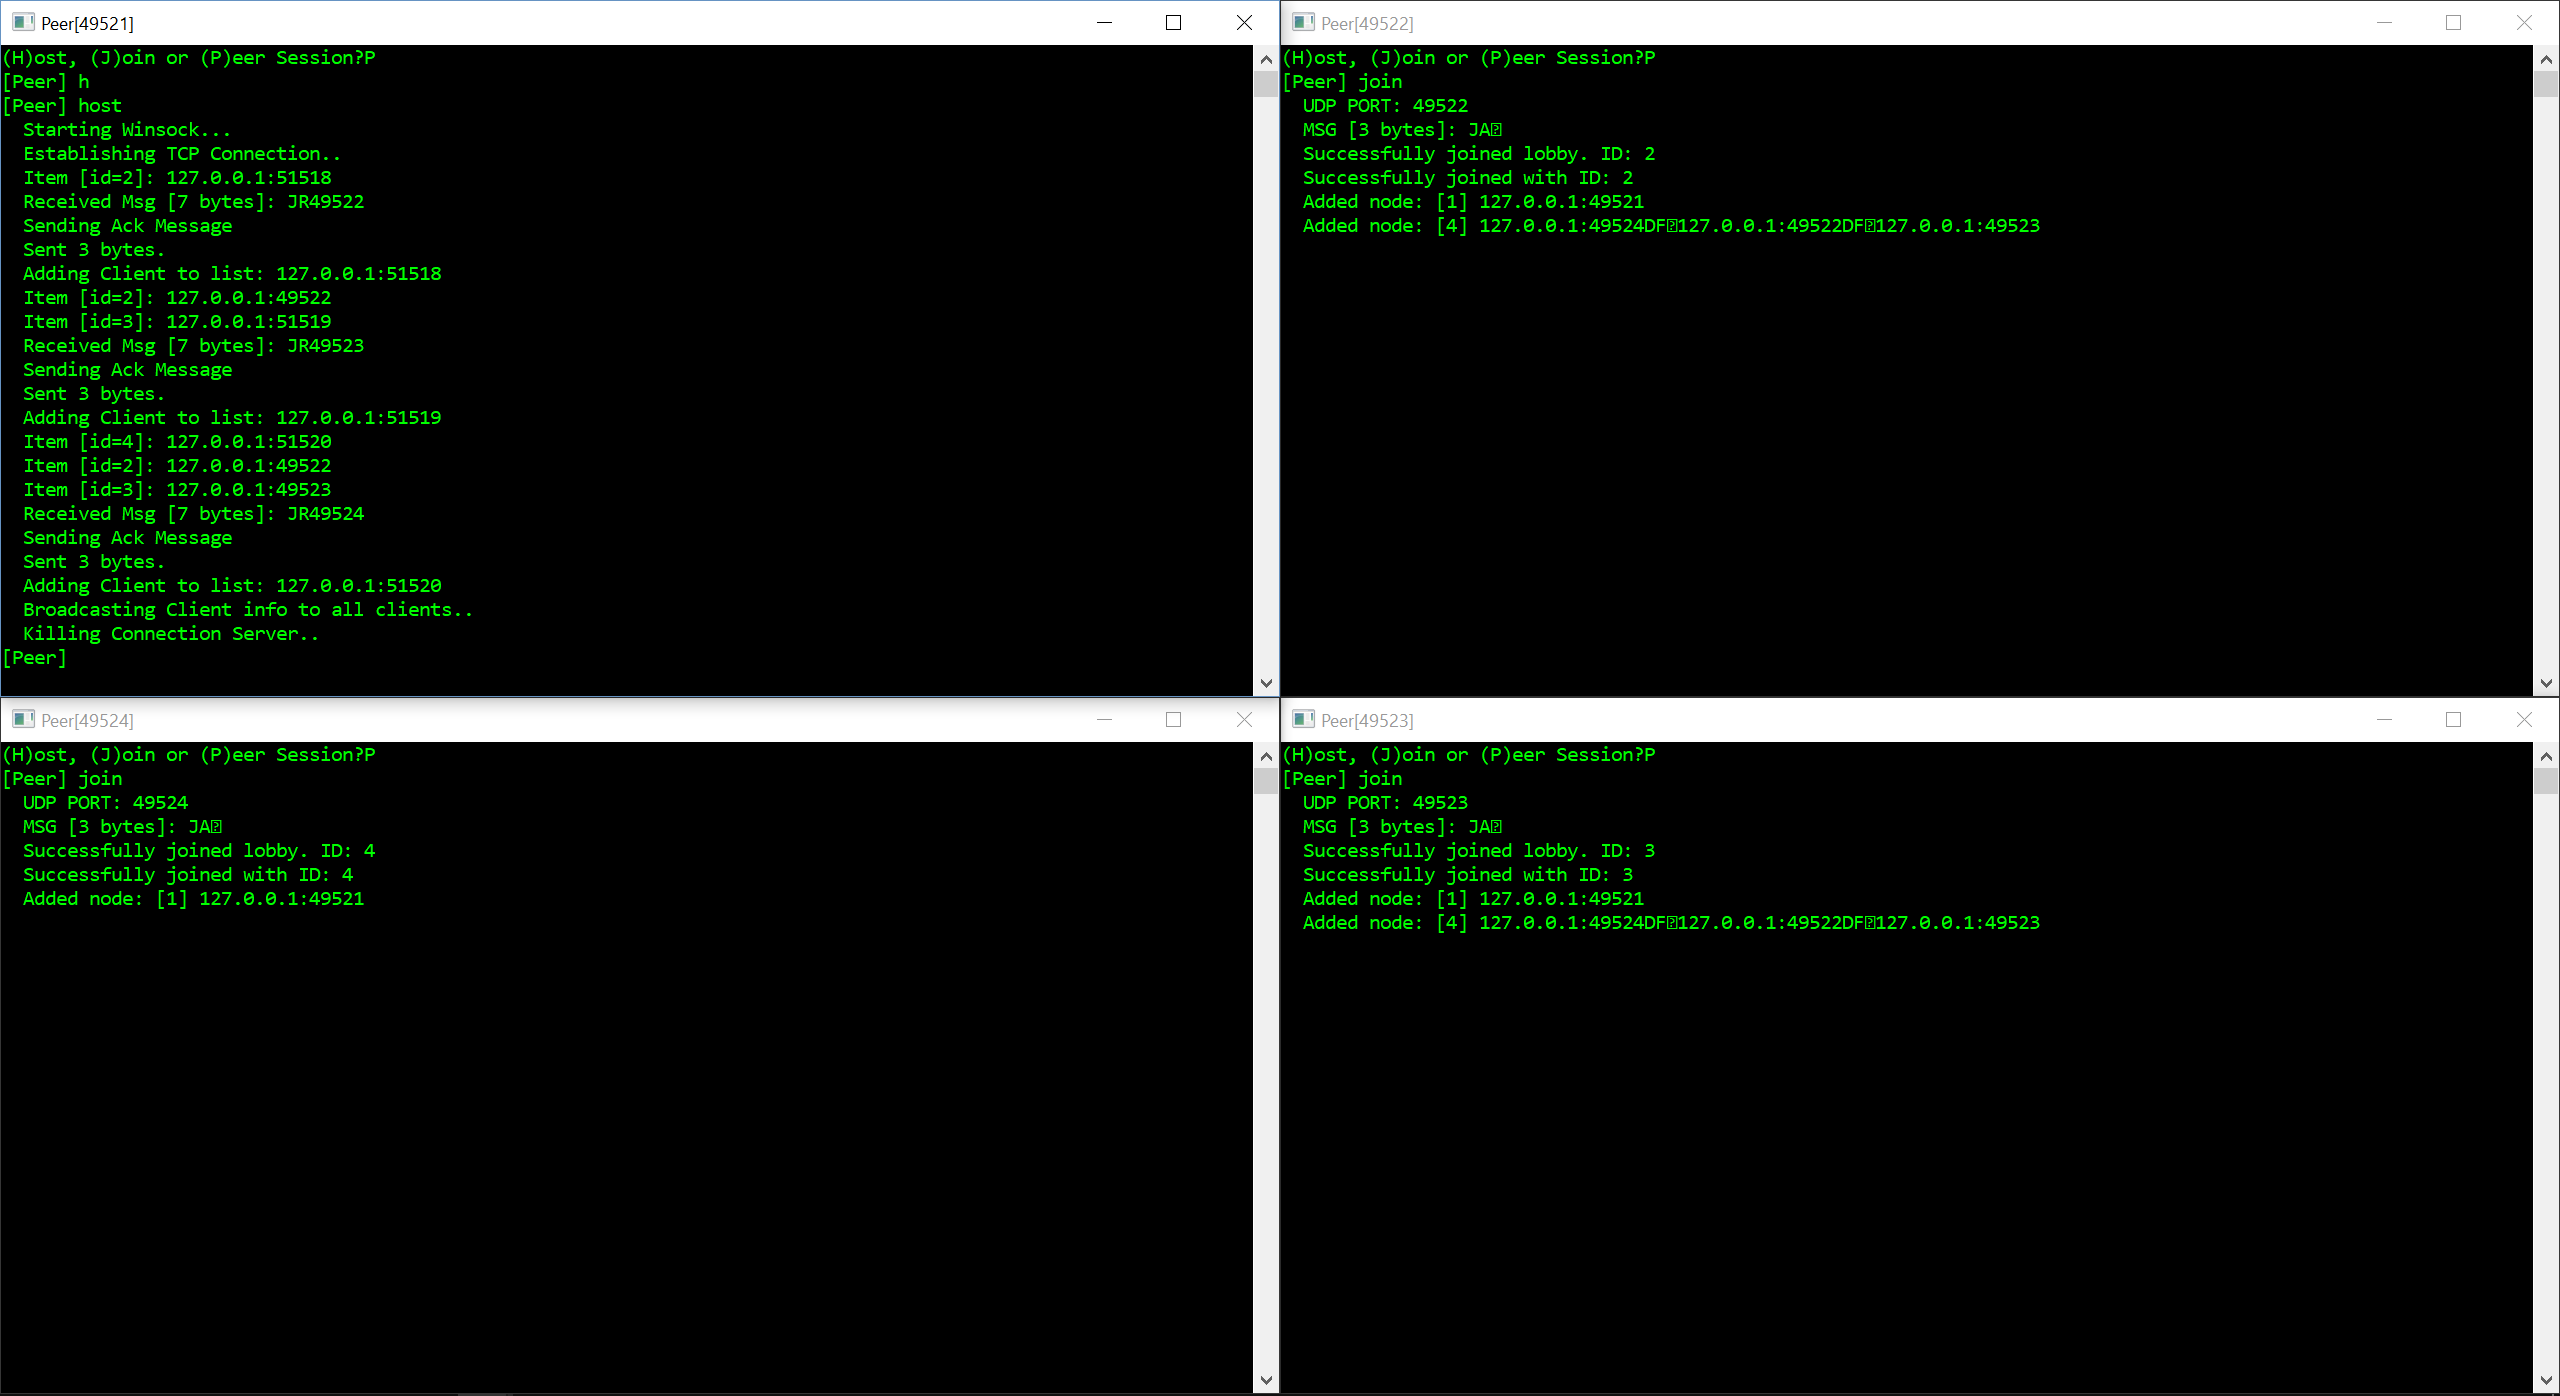
\includegraphics[width=\textwidth]{GNAT/sending_too_fast.png}
  \caption{Messages being broadcast with no delay}
  \label{fig:broadcast_too_fast}
\end{figure}

\begin{figure}[!h]
  \centering
  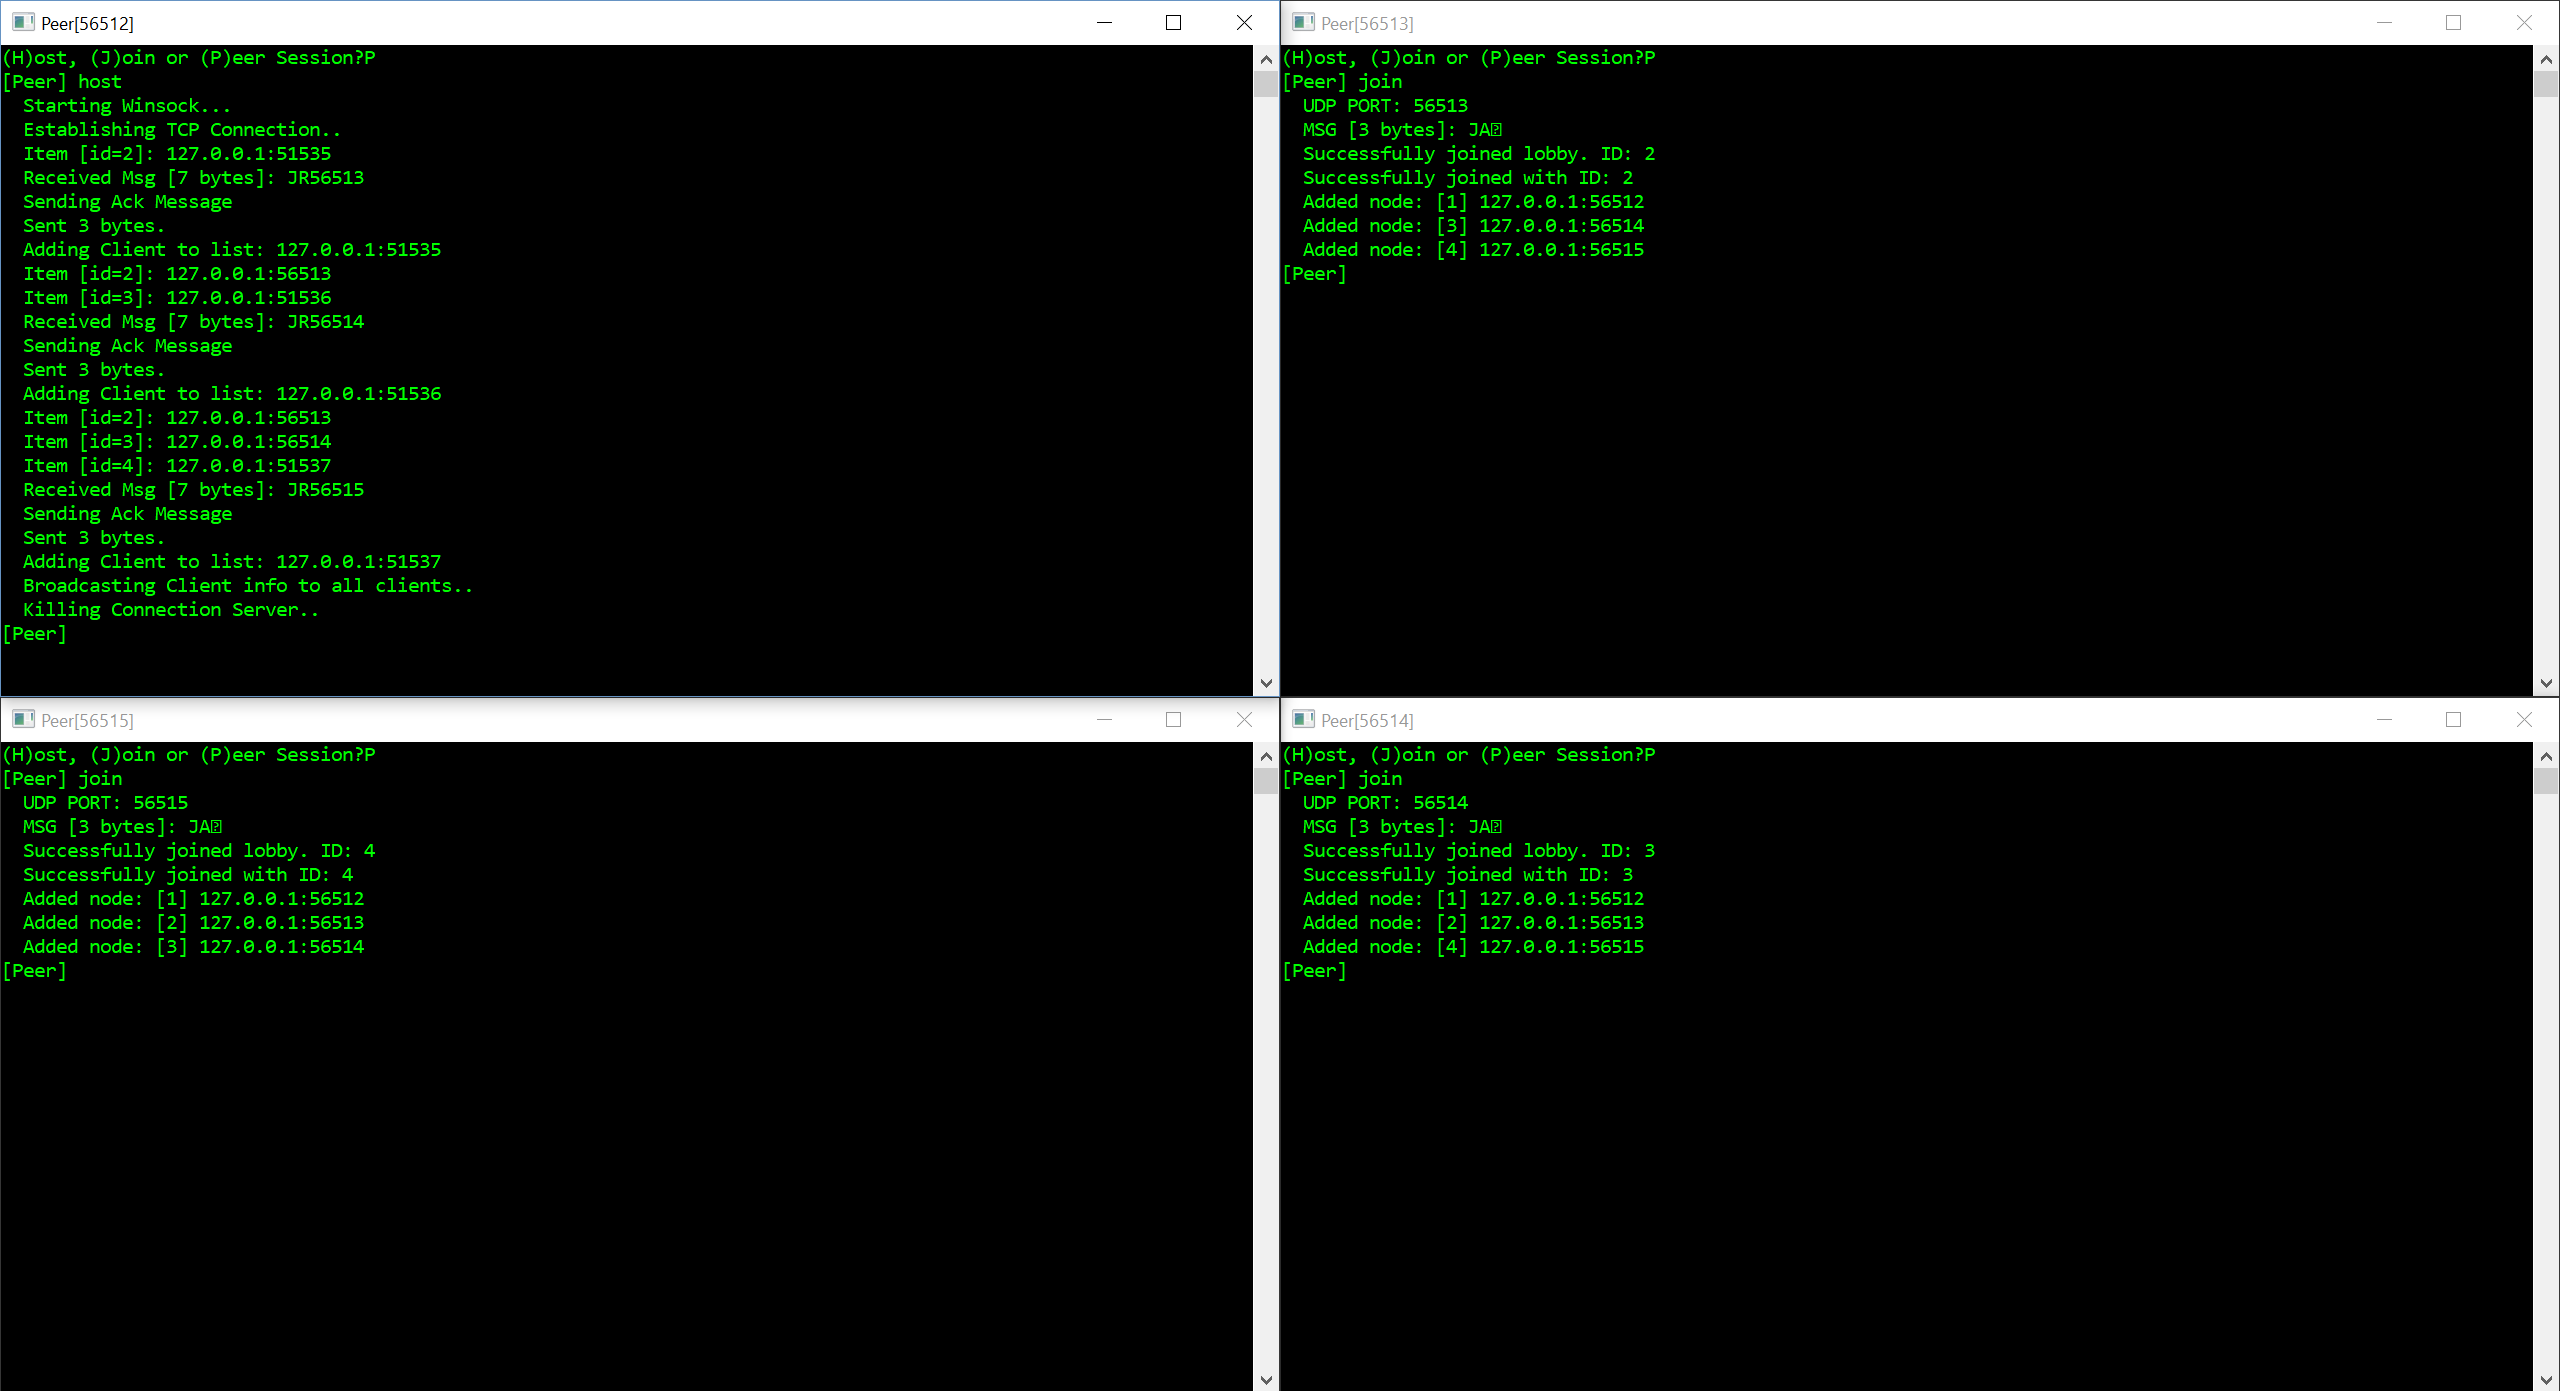
\includegraphics[width=\textwidth]{GNAT/sending_with_delay.png}
  \caption{Messages being broadcast with delay}
  \label{fig:broadcast_with_delay}
\end{figure}

\chapter{GNAT Code Snippets}

\section{Pre-compiled Headers}
When developing a project that uses code that will not change, such as the std library and winsock, it is inefficient to compile the code for these libraries every time the project code is compiled. To greatly improve compile times, precompiled headers are used.

\textbf{pch.h}
\begin{lstlisting}
// General
#include <string>
#include <iostream>
#include <thread>

// Data Structures
#include <map>
#include <vector>

// WinSock
#include <winsock2.h>
#include <Ws2tcpip.h>
#include <windows.h>

#pragma comment (lib, "ws2_32.lib")

// Custom
#include "log.h"
\end{lstlisting}

\textbf{pch.cpp}
\begin{lstlisting}
#include "pch.h"
\end{lstlisting}







\section{Logging library wrapper}
For the logging library, a 3rd party project was used called spdlog. The wrapper is used to use this library in predefined ways.


\textbf{Log.h}
\begin{lstlisting}
#pragma once
#include <memory>
#include <spdlog/spdlog.h>

namespace GNAT {
	class GNAT_Log {
	public:
		static void init();
		static void init_client();
		static void init_server();
		static void init_peer();
		static void init_connection();

		inline static std::shared_ptr<spdlog::logger>& getConnectionLogger() { return connection_logger; }
		inline static std::shared_ptr<spdlog::logger>& getServerLogger() { return server_logger; }
		inline static std::shared_ptr<spdlog::logger>& getPeerLogger() { return peer_logger; }
		inline static std::shared_ptr<spdlog::logger>& getClientLogger() { return client_logger; }

	private:
		const static int LOG_FILE_SIZE_IN_MB = 5;
		const static int ROTATING_FILE_COUNT = 3;

		static std::shared_ptr<spdlog::logger> connection_logger;
		static std::shared_ptr<spdlog::logger> server_logger;
		static std::shared_ptr<spdlog::logger> peer_logger;
		static std::shared_ptr<spdlog::logger> client_logger;
	};
}

// Loging Macros
#define CONNECT_LOG_FATAL(...) GNAT::GNAT_Log::getConnectionLogger()->fatal(__VA_ARGS__); std::cout << "  " << __VA_ARGS__ << std::endl
#define CONNECT_LOG_ERROR(...) GNAT::GNAT_Log::getConnectionLogger()->error(__VA_ARGS__); std::cout << "  " << __VA_ARGS__ << std::endl
#define CONNECT_LOG_WARN(...) GNAT::GNAT_Log::getConnectionLogger()->warn(__VA_ARGS__);	 std::cout << "  " << __VA_ARGS__ << std::endl
#define CONNECT_LOG_INFO(...) GNAT::GNAT_Log::getConnectionLogger()->info(__VA_ARGS__);	 std::cout << "  " << __VA_ARGS__ << std::endl
#define CONNECT_LOG_TRACE(...) GNAT::GNAT_Log::getConnectionLogger()->trace(__VA_ARGS__); std::cout << "  " << __VA_ARGS__ << std::endl

#define SERVER_LOG_FATAL(...) GNAT::GNAT_Log::getServerLogger()->fatal(__VA_ARGS__); std::cout << "  " << __VA_ARGS__ << std::endl
#define SERVER_LOG_ERROR(...) GNAT::GNAT_Log::getServerLogger()->error(__VA_ARGS__); std::cout << "  " << __VA_ARGS__ << std::endl
#define SERVER_LOG_WARN(...) GNAT::GNAT_Log::getServerLogger()->warn(__VA_ARGS__);	 std::cout << "  " << __VA_ARGS__ << std::endl
#define SERVER_LOG_INFO(...) GNAT::GNAT_Log::getServerLogger()->info(__VA_ARGS__);	 std::cout << "  " << __VA_ARGS__ << std::endl
#define SERVER_LOG_TRACE(...) GNAT::GNAT_Log::getServerLogger()->trace(__VA_ARGS__); std::cout << "  " << __VA_ARGS__ << std::endl

#define PEER_LOG_FATAL(...) GNAT::GNAT_Log::getPeerLogger()->fatal(__VA_ARGS__);	 std::cout << "  " << __VA_ARGS__ << std::endl
#define PEER_LOG_ERROR(...) GNAT::GNAT_Log::getPeerLogger()->error(__VA_ARGS__);	 std::cout << "  " << __VA_ARGS__ << std::endl
#define PEER_LOG_WARN(...) GNAT::GNAT_Log::getPeerLogger()->warn(__VA_ARGS__);		 std::cout << "  " << __VA_ARGS__ << std::endl
#define PEER_LOG_INFO(...) GNAT::GNAT_Log::getPeerLogger()->info(__VA_ARGS__);		 std::cout << "  " << __VA_ARGS__ << std::endl
#define PEER_LOG_TRACE(...) GNAT::GNAT_Log::getPeerLogger()->trace(__VA_ARGS__);	 std::cout << "  " << __VA_ARGS__ << std::endl

#define CLIENT_LOG_FATAL(...) GNAT::GNAT_Log::getClientLogger()->fatal(__VA_ARGS__); std::cout << "  " << __VA_ARGS__ << std::endl
#define CLIENT_LOG_ERROR(...) GNAT::GNAT_Log::getClientLogger()->error(__VA_ARGS__); std::cout << "  " << __VA_ARGS__ << std::endl
#define CLIENT_LOG_WARN(...) GNAT::GNAT_Log::getClientLogger()->warn(__VA_ARGS__);	 std::cout << "  " << __VA_ARGS__ << std::endl
#define CLIENT_LOG_INFO(...) GNAT::GNAT_Log::getClientLogger()->info(__VA_ARGS__);	 std::cout << "  " << __VA_ARGS__ << std::endl
#define CLIENT_LOG_TRACE(...) GNAT::GNAT_Log::getClientLogger()->trace(__VA_ARGS__); std::cout << "  " << __VA_ARGS__ << std::endl
\end{lstlisting}

\textbf{Log.cpp}

\begin{lstlisting}
#include "pch.h"
#include "log.h"
#include <spdlog/sinks/rotating_file_sink.h>
#include <ctime>

namespace GNAT {
	std::shared_ptr<spdlog::logger> GNAT_Log::connection_logger;
	std::shared_ptr<spdlog::logger> GNAT_Log::server_logger;
	std::shared_ptr<spdlog::logger> GNAT_Log::peer_logger;
	std::shared_ptr<spdlog::logger> GNAT_Log::client_logger;

	void GNAT_Log::init() {
		spdlog::set_pattern("%^[%T] %n: %v%$");

		try
		{
			peer_logger = spdlog::rotating_logger_mt("CONN", "Logs\\CONN-" + std::to_string(std::time(0)) + ".log", 1024 * 1024 * LOG_FILE_SIZE_IN_MB, ROTATING_FILE_COUNT);
			server_logger = spdlog::rotating_logger_mt("SERV", "Logs\\SERV-" + std::to_string(std::time(0)) + ".log", 1024 * 1024 * LOG_FILE_SIZE_IN_MB, ROTATING_FILE_COUNT);
			peer_logger = spdlog::rotating_logger_mt("PEER", "Logs\\PEER-" + std::to_string(std::time(0)) + ".log", 1024 * 1024 * LOG_FILE_SIZE_IN_MB, ROTATING_FILE_COUNT);
			client_logger = spdlog::rotating_logger_mt("CLNT", "Logs\\CLNT-" + std::to_string(std::time(0)) + ".log", 1024 * 1024 * LOG_FILE_SIZE_IN_MB, ROTATING_FILE_COUNT);
		}
		catch (const spdlog::spdlog_ex& ex)
		{
			std::cout << "Log initialization failed: " << ex.what() << std::endl;
		}
	}

	void GNAT_Log::init_client() {
		spdlog::set_pattern("%^[%T] %n: %v%$");

		try
		{
			client_logger = spdlog::rotating_logger_mt("CLNT", "Logs\\CLNT-" + std::to_string(std::time(0)) + ".log", 1024 * 1024 * LOG_FILE_SIZE_IN_MB, ROTATING_FILE_COUNT);
		}
		catch (const spdlog::spdlog_ex& ex)
		{
			std::cout << "Log initialization failed: " << ex.what() << std::endl;
		}
	}

	void GNAT_Log::init_server() {
		spdlog::set_pattern("%^[%T] %n: %v%$");

		try
		{
			server_logger = spdlog::rotating_logger_mt("SERV", "Logs\\SERV-" + std::to_string(std::time(0)) + ".log", 1024 * 1024 * LOG_FILE_SIZE_IN_MB, ROTATING_FILE_COUNT);
		}
		catch (const spdlog::spdlog_ex& ex)
		{
			std::cout << "Log initialization failed: " << ex.what() << std::endl;
		}
	}

	void GNAT_Log::init_peer() {
		spdlog::set_pattern("%^[%T] %n: %v%$");

		try
		{
			peer_logger = spdlog::rotating_logger_mt("PEER", "Logs\\PEER-" + std::to_string(std::time(0)) + ".log", 1024 * 1024 * LOG_FILE_SIZE_IN_MB, ROTATING_FILE_COUNT);
		}
		catch (const spdlog::spdlog_ex& ex)
		{
			std::cout << "Log initialization failed: " << ex.what() << std::endl;
		}
	}

	void GNAT_Log::init_connection() {
		spdlog::set_pattern("%^[%T] %n: %v%$");

		try
		{
			connection_logger = spdlog::rotating_logger_mt("CONN", "Logs\\CONN-" + std::to_string(std::time(0)) + ".log", 1024 * 1024 * LOG_FILE_SIZE_IN_MB, ROTATING_FILE_COUNT);
		}
		catch (const spdlog::spdlog_ex& ex)
		{
			std::cout << "Log initialization failed: " << ex.what() << std::endl;
		}
	}
}
\end{lstlisting}
